\documentclass[12pt]{article}

\usepackage{hyperref}
\usepackage[width=6in,height=8in]{geometry}
\usepackage{guitardiagrams}
\usepackage{graphicx}
\usepackage{float}

\usepackage{pdfpages}


\usepackage{amsthm}
\theoremstyle{definition}
\newtheorem{exercise}{Exercise}


\title{D Major Scale - Open Position}
\author{Addison Ballif}
\date{\today}

\begin{document}

\maketitle

Here are all the notes of the D Major scale in open position.

\fretboard[frets=4]{
    1/0/{E},
    1/2/{F$\sharp$},
    1/3/{G},
    2/0/{A},
    2/2/{B},
    2/4/{C$\sharp$},
    3/0/{D},
    3/2/{E},
    3/4/{F$\sharp$},
    4/0/{G},
    4/2/{A},
    5/0/{B},
    5/2/{C$\sharp$},
    5/3/{D},
    6/0/{E},
    6/2/{F$\sharp$},
    6/3/{G}
}
\begin{center}
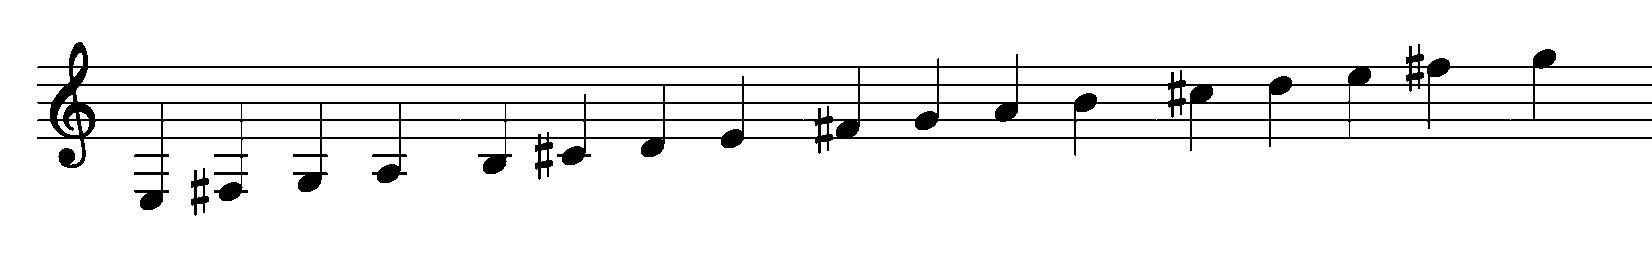
\includegraphics[width=\linewidth]{fig01.png}
\end{center}

You can play this scale with one finger per fret. Let your index finger cover all the 2nd fret notes, your middle finger cover all the 3rd fret notes, and your ring finger cover all the 4th fret notes. 

Practice this against a drone. \footnote{A drone can be found on my website \href{https://ahballif.github.io/AddisonGuitarResources/drones.html}{here}. This website also has a metronome if needed. }
It is also important to practice this scale with a metronome. Set the metronome slow (under 100) and play quarter notes. 
Once you are comfortable you can change to eighth notes (two notes per click). 

If using a pick, use alternate picking starting with a down stroke (towards the ground). 



\end{document}
